% !!!IMPORTANT NOTE: Please read carefully all information including those preceded by % sign
%Before you compile the tex file please download the class file AIMS.cls from the following URL link to the
%local folder where your tex file resides. http://aimsciences.org/journals/tex-sample/AIMS.cls.
\documentclass{aims}
\usepackage{amsmath,tikz}
\usepackage{paralist}
\usetikzlibrary{matrix}
\usepackage{graphics} %% add this and next lines if pictures should be in esp format
\usepackage{epsfig} %For pictures: screened artwork should be set up with an 85 or 100 line screen
\usepackage{graphicx}  \usepackage{epstopdf}%This is to transfer .eps figure to .pdf figure; please compile your paper using PDFLeTex or PDFTeXify.
\usepackage{amssymb}
\usepackage{amsthm}
% \usepackage{graphicx}
% \usepackage{pictex}
% \usepackage{pst-all}
\usepackage{epstopdf}
\usepackage{verbatim}
% \usepackage{frontespizio}
% \usepackage{flafter}% per float
\epstopdfsetup{update}
%\usepackage{makeidx}
\usepackage{mathrsfs}
\usepackage{mathtools}
\usepackage{pstricks}
\usepackage{subcaption}
\usepackage[percent]{overpic}
%\usepackage{refcheck}
\usepackage[colorlinks=true]{hyperref}
% Warning: when you first run your tex file, some errors might occur,
% please just press enter key to end the compilation process, then it will be fine if you run your tex file again.
% Note that it is highly recommended by AIMS to use this package.
\hypersetup{urlcolor=blue, citecolor=red}
%\usepackage{hyperref}

\textheight=8.2 true in
\textwidth=5.0 true in
\topmargin 30pt
\setcounter{page}{1}

% The next 5 line will be entered by an editorial staff.
\def\currentvolume{X}
\def\currentissue{X}
\def\currentyear{200X}
\def\currentmonth{XX}
\def\ppages{X--XX}
\def\DOI{10.3934/xx.xx.xx.xx}

% Please minimize the usage of "newtheorem", "newcommand", and use
% equation numbers only situation when they provide essential convenience
% Try to avoid defining your own macros

\newtheorem{theorem}{Theorem}[section]
\newtheorem{corollary}{Corollary}
\newtheorem*{main}{Main Theorem}
\newtheorem{lemma}[theorem]{Lemma}
\newtheorem{proposition}{Proposition}
\newtheorem{conjecture}{Conjecture}
\newtheorem*{problem}{Problem}
\theoremstyle{definition}
\newtheorem{definition}[theorem]{Definition}
\newtheorem{remark}{Remark}
\newtheorem*{notation}{Notation}
\newcommand{\ep}{\varepsilon}
\newcommand{\eps}[1]{{#1}_{\varepsilon}}


%% Place the running title of the paper with 40 letters or less in []
%% and the full title of the paper in { }.
\title[DyCon blog post] %Use the shortened version of the full title
{DyCon blog post}

% Place all authors' names in [ ] shown as running head, Leave { } empty
% Please use `and' to connect the last two names if applicable
% Use FirstNameInitial.  MiddleNameInitial. LastName, or only last names of authors if there are too many authors
%\author[Dario Pighin and Enrique Zuazua]{}

% It is required to enter 2010 MSC.
%\subjclass{Primary: 58F15, 58F17; Secondary: 53C35.}[ADD]
% Please provide minimum  5 keywords.
% \keywords{Dimension theory, Poincar\'e recurrences, multifractal analysis.}[ADD]

% Email address of each of all authors is required.
% You may list email addresses of all other authors, separately.
% \email{dario.pighin@uam.es}
% \email{enrique.zuazua@uam.es}

% Put your short thanks below. For long thanks/acknowlegements,
%please go to the last acknowlegments section.
%\thanks{This work was partially supported by the Advanced Grant DYCON (Dynamic Control) of the European Research Council Executive Agency, FA9550-15-1-0027 of AFOSR, FA9550-14-1-0214 of the EOARD-AFOSR, the MTM2014-52347 Grant of the MINECO (Spain) and ICON of the French ANR}
%[ADD]

% Add corresponding author at the footnote of the first page if it is necessary. 
% Plase add $^*$ adjacent to the corresponding author's name on the first page. 
% The example shown in this template is if the first author is the corresponding author.
%\thanks{$^*$ Corresponding author: xxxx}[ADD]

\begin{document}
	\maketitle
	
	%% Enter the first author's name and address:
	%\centerline{\scshape Dario Pighin$^*$}
	%\medskip
	%{\footnotesize
	%% please put the address of the first author
	% \centerline{Departamento de Matem\'aticas, Universidad Aut\'onoma de Madrid}
	%%   \centerline{Other lines}
	%   \centerline{28049 Madrid, Spain}
	%} % Do not forget to end the {\footnotesize by the sign }
	%
	%
	%\medskip
	%
	%\centerline{\scshape Enrique Zuazua}
	%\medskip
	%{\footnotesize
	%	% please put the address of the first author
	%	\centerline{DeustoTech, Fundaci\'on Deusto}
	%	%   \centerline{Other lines}
	%	\centerline{Avda. Universidades,
	%		24, 48007, Bilbao, Basque Country, Spain}
	%} % Do not forget to end the {\footnotesize by the sign }
	%\medskip
	%{\footnotesize
	%	% please put the address of the first author
	%	\centerline{Departamento de Matem\'aticas, Universidad Aut\'onoma de Madrid}
	%	%   \centerline{Other lines}
	%	\centerline{28049 Madrid, Spain}
	%} % Do not forget to end the {\footnotesize by the sign }
	%\medskip
	%{\footnotesize
	%	% please put the address of the first author
	%	\centerline{Facultad de Ingenier\'ia, Universidad de Deusto}
	%	%   \centerline{Other lines}
	%	\centerline{Avda. Universidades,
	%		24, 48007, Bilbao, Basque Country, Spain}
	%} % Do not forget to end the {\footnotesize by the sign }
	%\medskip
	%{\footnotesize
	%	% please put the address of the first author
	%	\centerline{Laboratoire Jacques-Louis Lions, UPMC Univ. Paris 06,}
	%	%   \centerline{Other lines}
	%	\centerline{CNRS–UMR 7598, Sorbonne Universit\'es, F-75005, Paris, France}
	%} % Do not forget to end the {\footnotesize by the sign }
	%
	%\bigskip
	%
	%% The name of the associate editor will be entered by an editorial staff
	%% "Communicated by the associate editor name" is not needed for special issue.
	%% \centerline{(Communicated by the associate editor name)}[ADD]
	%
	%
	%%The abstract of your paper
	%\begin{abstract}
	%
	%
	%\end{abstract}
	%\medskip
	%{\center{\textit{Dedicated to professor Jiongmin Yong on the occasion of his 60th birthday}}}
	%\medskip
	
	%The title of your section 1
	Consider a rotor, rotating about a fixed axis $z$. Assume that, because of wear and damage, the mass distribution is not homogeneous. This leads to dangerous vibrations in the rotation. A prototypical example can be a wind turbine, which is often affected by misalignment of the blades and/or mass imbalance of the hub and blades \cite{jeffrey2012method}.
	
	Two balancing heads are mounted at the endpoints of the axle, as in figure \ref{spindlegrinder8mod}. Each balancing head is made of two masses free to rotate to compensate the imbalance.
	%In the preprint \cite{RIO}
	Our goal is to employ control theoretical techniques to to minimize the vibrations, moving the balancing masses.
	
	\begin{figure}[htp]
		\begin{center}
			% Requires \usepackage{graphicx}
			% replace aims_logo.eps by your figure file name
			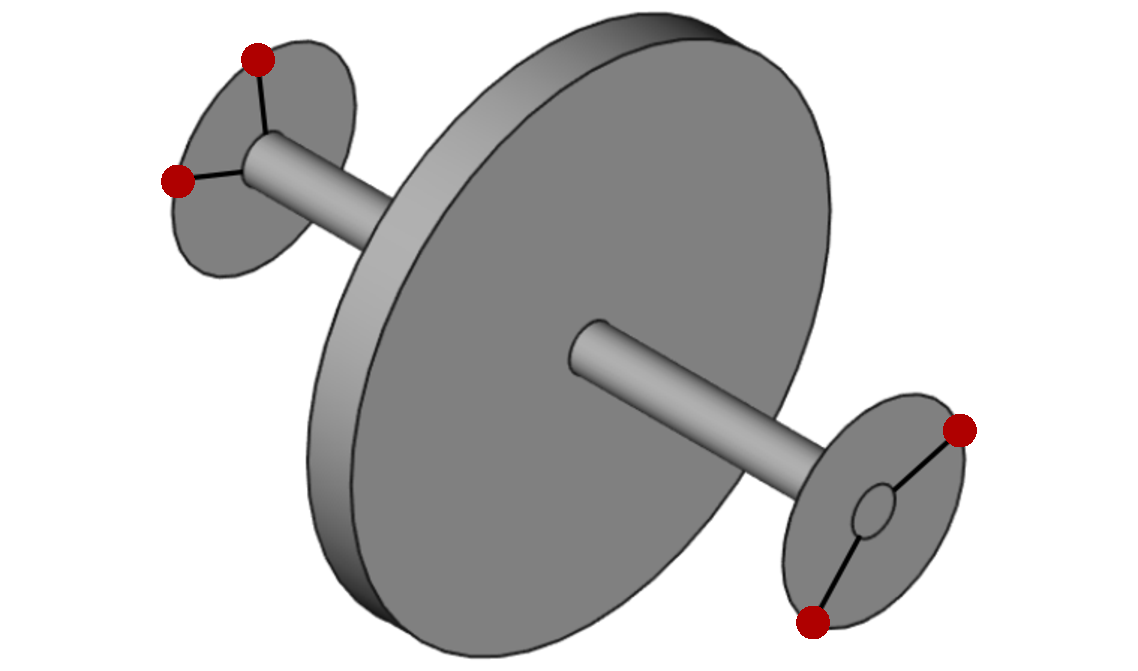
\includegraphics[width=6cm]{spindlegrinder8mod.pdf}\\
			\caption{The rotor and the balancing device are represented. In the special case represented, the balancing heads are located at the endpoints of the spindle. The four balancing masses (two for each balancing head) are drawn in red.}
			\label{spindlegrinder8mod}
		\end{center}
	\end{figure}
	
	Suppose the rotor is a rigid body rotating about a fixed axis. The angular velocity $\omega$ is assumed constant.
	
	Consider $(O;(x,y,z))$ rotor-fixed reference frame.
	
	\begin{figure}
		\begin{overpic}[scale=0.35]{spindlegrinder7_frontmodmeasnew.png}
			\put (-3.85, 24.0) {$r_2$}
			\put (98.85, 24.0) {$r_1$}
			\put (30, 3.0) {$b$}
			\put (68, 3.0) {$a$}
		\end{overpic}
		\caption{Front view of the system made of rotor and balancing device.}
		\label{spindlegrinder7_frontmodmeasnew}
	\end{figure}
	
	\begin{figure}
		\centering
		\begin{subfigure}{.6\textwidth}
			\centering
			\includegraphics[width=.5\linewidth]{"angles6".pdf}
			\caption{\textit{intermediate} angle}
			\label{fig:sub1}
		\end{subfigure}%
		\begin{subfigure}{.6\textwidth}
			\centering
			\includegraphics[width=.5\linewidth]{"angles5".pdf}
			\caption{\textit{gap} angle}
			\label{fig:sub2}
		\end{subfigure}
		\caption{One balancing head is considered. The balancing masses $(m_i,P_{i,1})$ and $(m_i,P_{i,2})$ are drawn in red. The bisector of the angle generated by $\overset{\longrightarrow}{OP_{i,1}}$ and $\overset{\longrightarrow}{OP_{i,2}}$ is the dashed line. The \textit{intermediate} angle $\alpha_i$ is represented in \ref{fig:sub1}, while the \textit{gap} angle $\gamma_i$ is depicted in \ref{fig:sub2}. The angles $\alpha_i$ and $\gamma_i$ give the position of the balancing masses in each balancing head.}\label{angle_grah_1}
	\end{figure}
	
	We consider two planes $\pi_1$ and $\pi_2$ orthogonal to the rotation axis $z$. The balancing device (see figures \ref{spindlegrinder8mod} and \ref{spindlegrinder7_frontmodmeasnew}) is made up two heads lying in each of these planes. The heads are integral with the rotor, whence they rotate together with the rotor. Each head is made of a pair of balancing masses, which are free to rotate orthogonally to the rotation axis $z$.  Namely, we have
	\begin{itemize}
		\item two planes $\pi_1\coloneqq \left\{z=-a\right\}$ and $\pi_2\coloneqq \left\{z=b\right\}$, with $a$, $b\geq 0$;
		%WARNING: We should put $(a,b)\in\mathbb{R}^2$.
		\item two mass-points $(m_1,P_{1,1})$ and $(m_1,P_{1,2})$ lying on $\pi_1$ at distance $r_1$ from the axis $z$, i.e., in the reference frame $(O;(x,y,z))$
		\begin{equation}\label{P1}
		\begin{cases}
		P_{1,1;x}=&r_1\cos(\alpha_1-\gamma_1)\\
		P_{1,1;y}=&r_1\sin(\alpha_1-\gamma_1)\\
		P_{1,1;z}=&-a,\\
		\end{cases}
		\hspace{0.3 cm}\mbox{and}\hspace{0.3 cm}
		\begin{cases}
		P_{1,2;x}=&r_1\cos(\alpha_1+\gamma_1)\\
		P_{1,2;y}=&r_1\sin(\alpha_1+\gamma_1)\\
		P_{1,2;z}=&-a;\\
		\end{cases}
		\end{equation}
		\item two mass-points $(m_2,P_{2,1})$ and $(m_2,P_{2,2})$ lying on $\pi_2$ at distance $r_2$ from the axis $z$, namely, in the reference frame $(O;(x,y,z))$
		\begin{equation}\label{P2}
		\begin{cases}
		P_{2,1;x}=&r_2\cos(\alpha_2-\gamma_2)\\
		P_{2,1;y}=&r_2\sin(\alpha_2-\gamma_2)\\
		P_{2,1;z}=&b,\\
		\end{cases}
		\hspace{0.3 cm}\mbox{and}\hspace{0.3 cm}
		\begin{cases}
		P_{2,2;x}=&r_2\cos(\alpha_2+\gamma_2)\\
		P_{2,2;y}=&r_2\sin(\alpha_2+\gamma_2)\\
		P_{2,2;z}=&b.\\
		\end{cases}
		\end{equation}
	\end{itemize}
	For any $i=1,2$, let $b_i$ be the bisector of the angle generated by $\overset{\longrightarrow}{OP_{i,1}}$ and $\overset{\longrightarrow}{OP_{i,2}}$ (see figure \ref{angle_grah_1}). For any $i=1,2$, the \textit{intermediate} angle $\alpha_i$ is the angle between the $x$-axis and the bisector $b_i$, while the \textit{gap} angle $\gamma_i$ is the angle between $\overset{\longrightarrow}{OP_{i,1}}$ and the bisector $b_i$.
	
	Note that the angles $\alpha_i$ and $\gamma_i$ are defined with respect to the rotor-fixed reference frame $(O;(x,y,z))$. Indeed, the balancing device described above is integral with the rotor.
	
	The imbalance is modelled by a resulting force $F$ and a momentum $N$ orthogonal to the rotation axis. In the rotor-fixed reference frame $(O;(x,y,z))$, set $P_1\coloneqq (0,0,-a)$, $P_2\coloneqq (0,0,b)$, $F\coloneqq (F_x,F_y,0)$ and $N\coloneqq (N_x,N_y,0)$. By imposing the equilibrium condition on forces and momenta, the force $F$ and the momentum $N$ can be decomposed into a force $F_1$ exerted at $P_1$ contained in plane $\pi_1$ and a force $F_2$ exerted at $P_2$ contained in $\pi_2$.
	
	In each plane, we generate a force to balance the system, by moving the balancing masses:
	\begin{itemize}
		\item in plane $\pi_1$, we compensate force $F_1$ by the centrifugal force:
		\begin{equation}\label{B_1}
		B_1=m_1r_1\omega^2\left(\cos(\alpha_1-\gamma_1)+\cos(\alpha_1+\gamma_1),\sin(\alpha_1-\gamma_1)+\sin(\alpha_1+\gamma_1)\right);
		\end{equation}
		\item in plane $\pi_2$, we compensate force $F_2$ by the centrifugal force:
		\begin{equation}\label{B_2}
		B_2=m_2r_2\omega^2\left(\cos(\alpha_2-\gamma_2)+\cos(\alpha_2+\gamma_2),\sin(\alpha_2-\gamma_2)+\sin(\alpha_2+\gamma_2)\right);	
		\end{equation}
	\end{itemize}
	
	The overall imbalance of the system is then given by the resulting force in $\pi_1$
	\begin{equation*}
	F_{ris,1}=B_1+F_1
	\end{equation*}
	and the resulting force in $\pi_2$
	\begin{equation*}
	F_{ris,2}=B_2+F_2.
	\end{equation*}
	
	The overall imbalance on the system made of rotor and balancing device is measured by imbalance indicator
	\begin{equation*}
	G=\|B_1+F_1\|^2+\|B_2+F_2\|^2.
	\end{equation*}
	
	By trigonometric formulas,
	$G:\mathbb{R}^4\longrightarrow \mathbb{R}$
	\begin{eqnarray}\label{G}
	G(\alpha_1,\gamma_1,\alpha_2,\gamma_2)&=&\left[\left|2m_1r_1\omega^2\cos(\gamma_1)\cos(\alpha_1)+F_{1,x}\right|^2\right.\\
	&\;&+\left|2m_1r_1\omega^2\cos(\gamma_1)\sin(\alpha_1)+F_{1,y}\right|^2\nonumber\\
	&\;&+\left|2m_2r_2\omega^2\cos(\gamma_2)\cos(\alpha_2)+F_{2,x}\right|^2\nonumber\\
	&\;&\left.+\left|2m_2r_2\omega^2\cos(\gamma_2)\sin(\alpha_2)+F_{2,y}\right|^2\right].\nonumber
	\end{eqnarray}
	
	Our task is to find a control strategy such that
	\begin{itemize}
		\item the balancing masses move from their initial configuration $\Phi_0$ to a final configuration $\overline{\Phi}$, where the imbalance is compensated;
		\item the imbalance and velocities should be kept small during the correction process.
	\end{itemize}
	
	We address the minimization problem
	\begin{equation}\label{functional}
	\min_{\Phi\in\mathscr{A}} \frac{1}{2}\int_0^{\infty} \left[\|\dot{\Phi}\|^2+{\beta}\hat{G}(\Phi)\right] dt,
	\end{equation}
	where
	\begin{equation}\label{admissible_trajectories}
	\mathscr{A}\coloneqq \left\{\Phi\in H^1_{loc}((0,+\infty);\mathbb{T}^4) \hspace{0.3 cm} \big| \hspace{0.3 cm} \Phi(0)=\Phi_0,\hspace{0.3 cm}\mbox{and}\hspace{0.3 cm}L(\Phi,\dot{\Phi})\in L^1(0,+\infty)\right\},
	\end{equation}
	with $H^1_{loc}((0,+\infty);\mathbb{T}^4)\coloneqq \cup_{T>0}H^1(0,T;\mathbb{T}^4)$. In \cite{RIO}, we obtained the following results:
	
	\begin{enumerate}
		\item there exists $\Phi\in \mathscr{A}$ minimizer of $J$;
		\item $\Phi=\left(\alpha_1,\gamma_1;\alpha_2,\gamma_2\right)$
		\begin{comment}
		$\in C^{\infty}([0,+\infty);\mathbb{T}^4)$
		\end{comment}
		is $C^{\infty}$ smooth and, for $i=1,2$, the following Euler-Lagrange equations are satisfied
		\begin{equation}\label{EL_new}
		\begin{cases}
		-\ddot{\alpha}_i=\beta\cos\left(\gamma_i\right)\left[-c^i_1\sin\left(\alpha_i\right)+c^i_2\cos\left(\alpha_i\right)\right]\hspace{0.6 cm}  &\mbox{in} \hspace{0.10 cm}(0,\infty)\\
		-\ddot{\gamma}_i=-\beta\sin\left(\gamma_i\right)\left[c^i_1\cos(\alpha_i)+c^i_2\sin(\alpha_i)-\cos(\gamma_i)\right]\hspace{0.6 cm}  &\mbox{in} \hspace{0.10 cm}(0,\infty)\\
		\alpha_i(0)=\alpha_{0,i},\hspace{0.16 cm}\gamma_i(0)=\gamma_{0,i}, \hspace{0.16 cm} \dot{\Phi}(T)\underset{T\to +\infty}{\longrightarrow}0.
		\end{cases}
		\end{equation}
		\item for any optimal trajectory $\Phi$ for \eqref{functional}, there exists $\overline{\Phi}\in\mathscr{S}$ such that
		\begin{equation}\label{prop_group_eq1}
		\Phi(t)\underset{t\to +\infty}{\longrightarrow}\overline{\Phi},
		\end{equation}
		\begin{equation}\label{prop_group_eq2}
		\dot{\Phi}(t)\underset{t\to +\infty}{\longrightarrow}0.
		\end{equation}
		and
		\begin{equation}\label{prop_group_eq3}
		\left|\hat{G}\left(\Phi(t)\right)\right|\underset{t\to +\infty}{\longrightarrow}0.
		\end{equation}
		If, in addition
		\begin{equation}\label{prop_group_eq4}
		m_1r_1 > \frac{\sqrt{F_{1,x}^2+F_{1,y}^2}}{2\omega^2}\hspace{0.3 cm}\mbox{and}\hspace{0.3 cm}m_2r_2> \frac{\sqrt{F_{2,x}^2+F_{2,y}^2}}{2\omega^2},
		\end{equation}
		we have the exponential estimate
		\begin{equation}\label{prop_group_eq6}
		\|\Phi(t)-\overline{\Phi}\|+\|\dot{\Phi}(t)\|+\left|G\left(\Phi(t)\right)\right|\leq C\exp\left(-\mu t\right),\hspace{0.3 cm}\forall \ t\geq 0,
		\end{equation}
		with $\mu >0$.
	\end{enumerate}
	
	We performed some numerical simulations, employing the expert interior-point optimization routine \verb!IPOpt! (see \cite{IDO} and \cite{waechter2009introduction}), the modelling language being \verb!AMPL! (see \cite{FAP}). The related code is available in the Appendix.
	
	In figures \ref{optcontrollab1}, \ref{optcontrollab2}, \ref{optcontrollab3} and \ref{optcontrollab4}, we plot a simulation, with initial datum\\
	$\Phi_0=\left(\alpha_{0,1},\gamma_{0,1};\alpha_{0,2},\gamma_{0,2}\right)\coloneqq \left(1,0.3,0.6,0.3\right)$. Condition \eqref{prop_group_eq4} is verified. In agreement with our result, the exponential stabilization emerges. In figure \ref{systemresponse}, we depict the imbalance indicator versus time along the computed trajectories. As expected, it decays to zero exponentially.
	
	
	
	\begin{figure}[htp]
		\begin{center}
			% Requires \usepackage{graphicx}
			% replace aims_logo.eps by your figure file name
			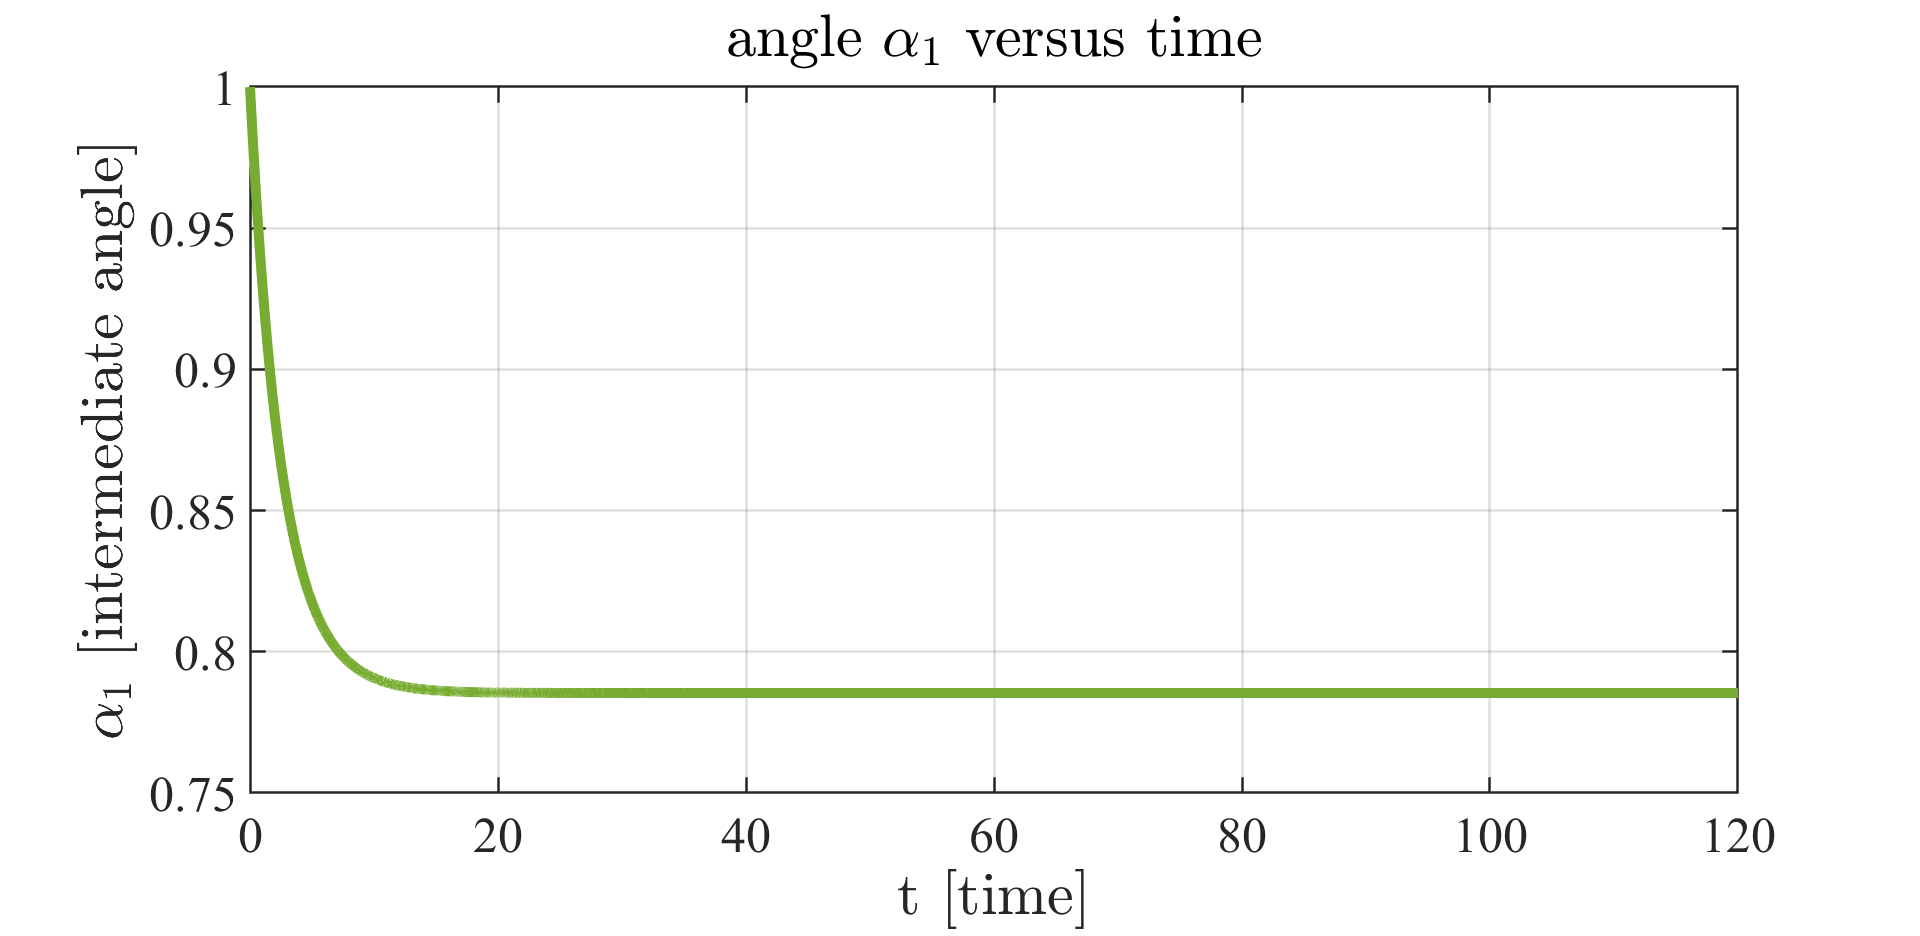
\includegraphics[width=11cm]{optstabilalpha1.png}\\
			\caption{Intermediate angle $\alpha_1$ versus time}
			\label{optcontrollab1}
		\end{center}
	\end{figure}
	
	\begin{figure}[htp]
		\begin{center}
			% Requires \usepackage{graphicx}
			% replace aims_logo.eps by your figure file name
			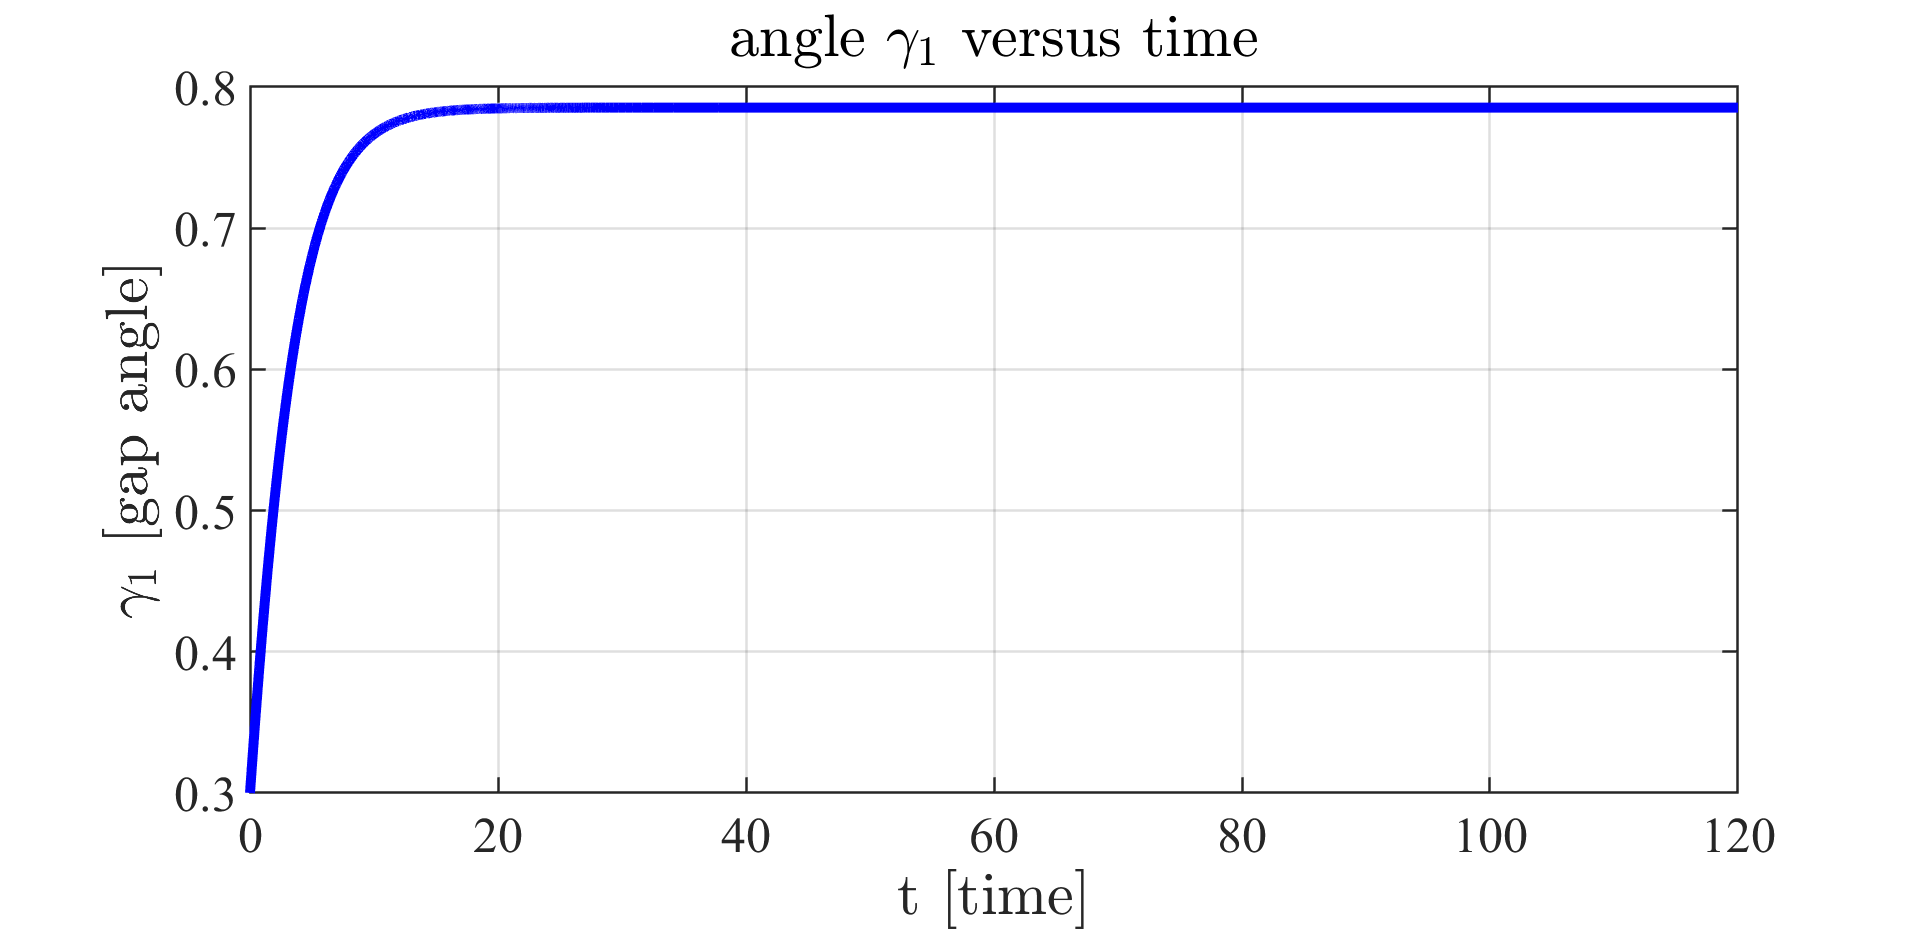
\includegraphics[width=11cm]{optstabilgamma1.png}\\
			\caption{Gap angle $\gamma_1$ versus time}
			\label{optcontrollab2}
		\end{center}
	\end{figure}
	
	\begin{figure}[htp]
		\begin{center}
			% Requires \usepackage{graphicx}
			% replace aims_logo.eps by your figure file name
			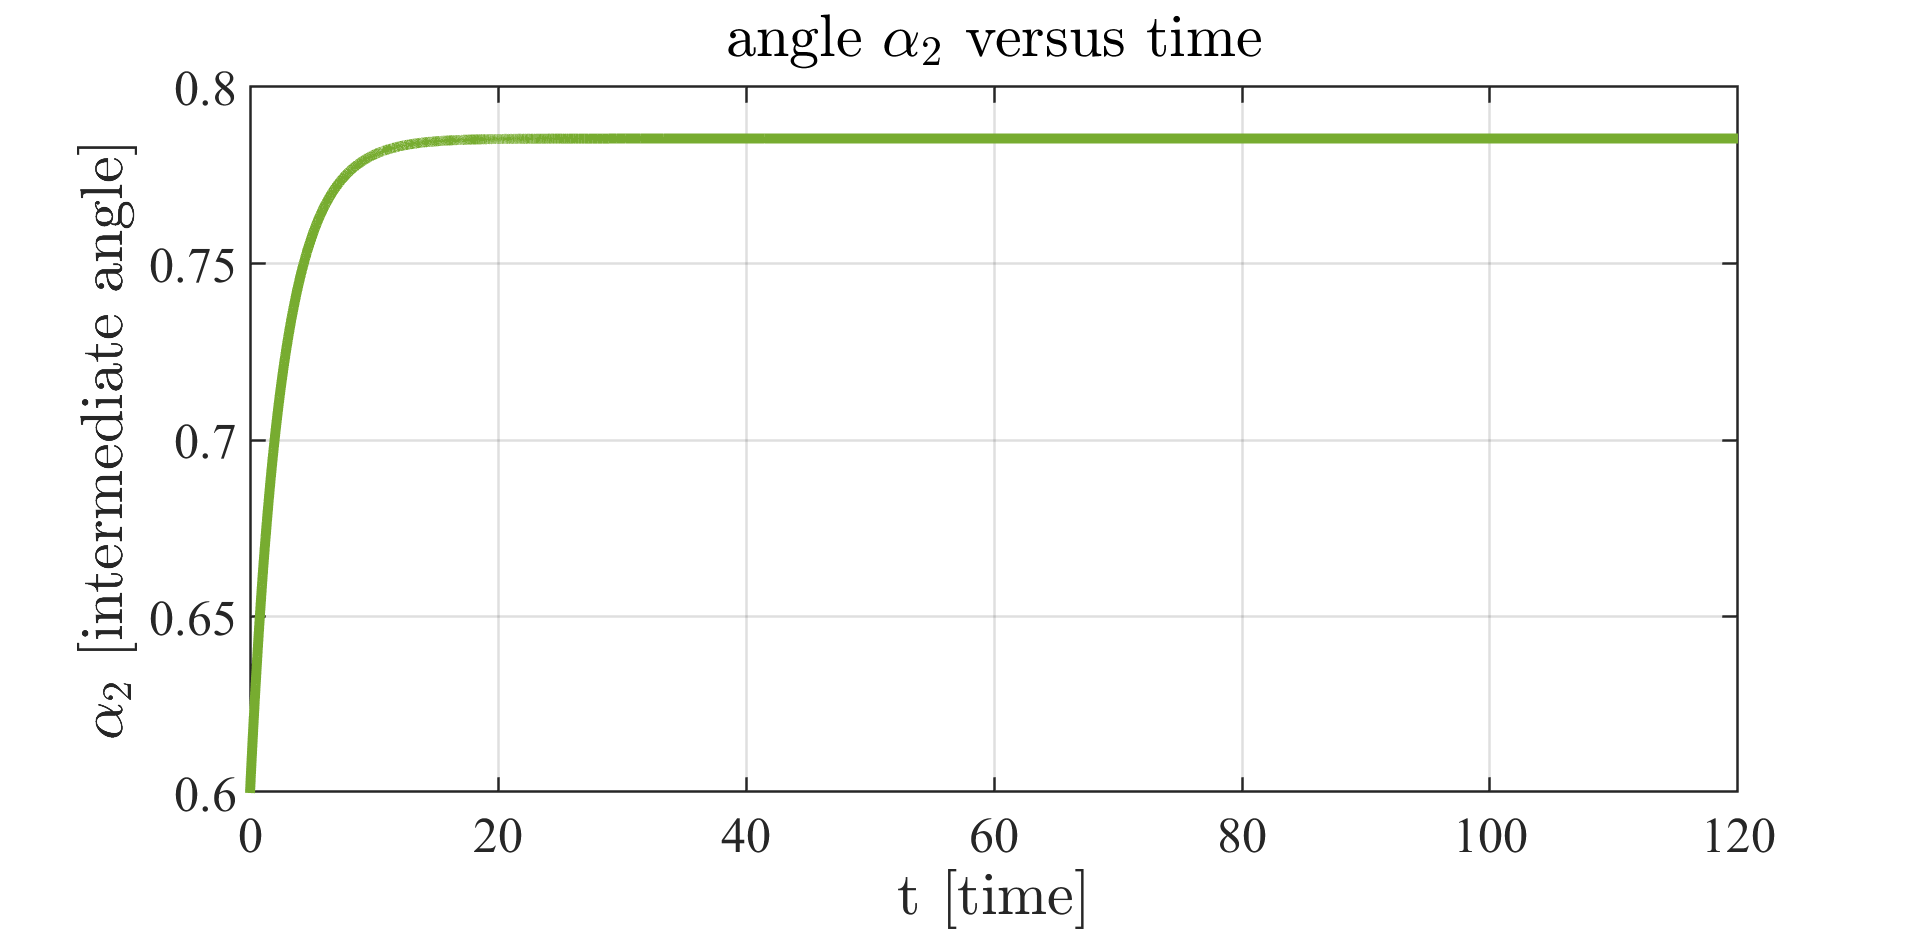
\includegraphics[width=11cm]{optstabilalpha2.png}\\
			\caption{Intermediate angle $\alpha_2$ versus time}
			\label{optcontrollab3}
		\end{center}
	\end{figure}
	
	\begin{figure}[htp]
		\begin{center}
			% Requires \usepackage{graphicx}
			% replace aims_logo.eps by your figure file name
			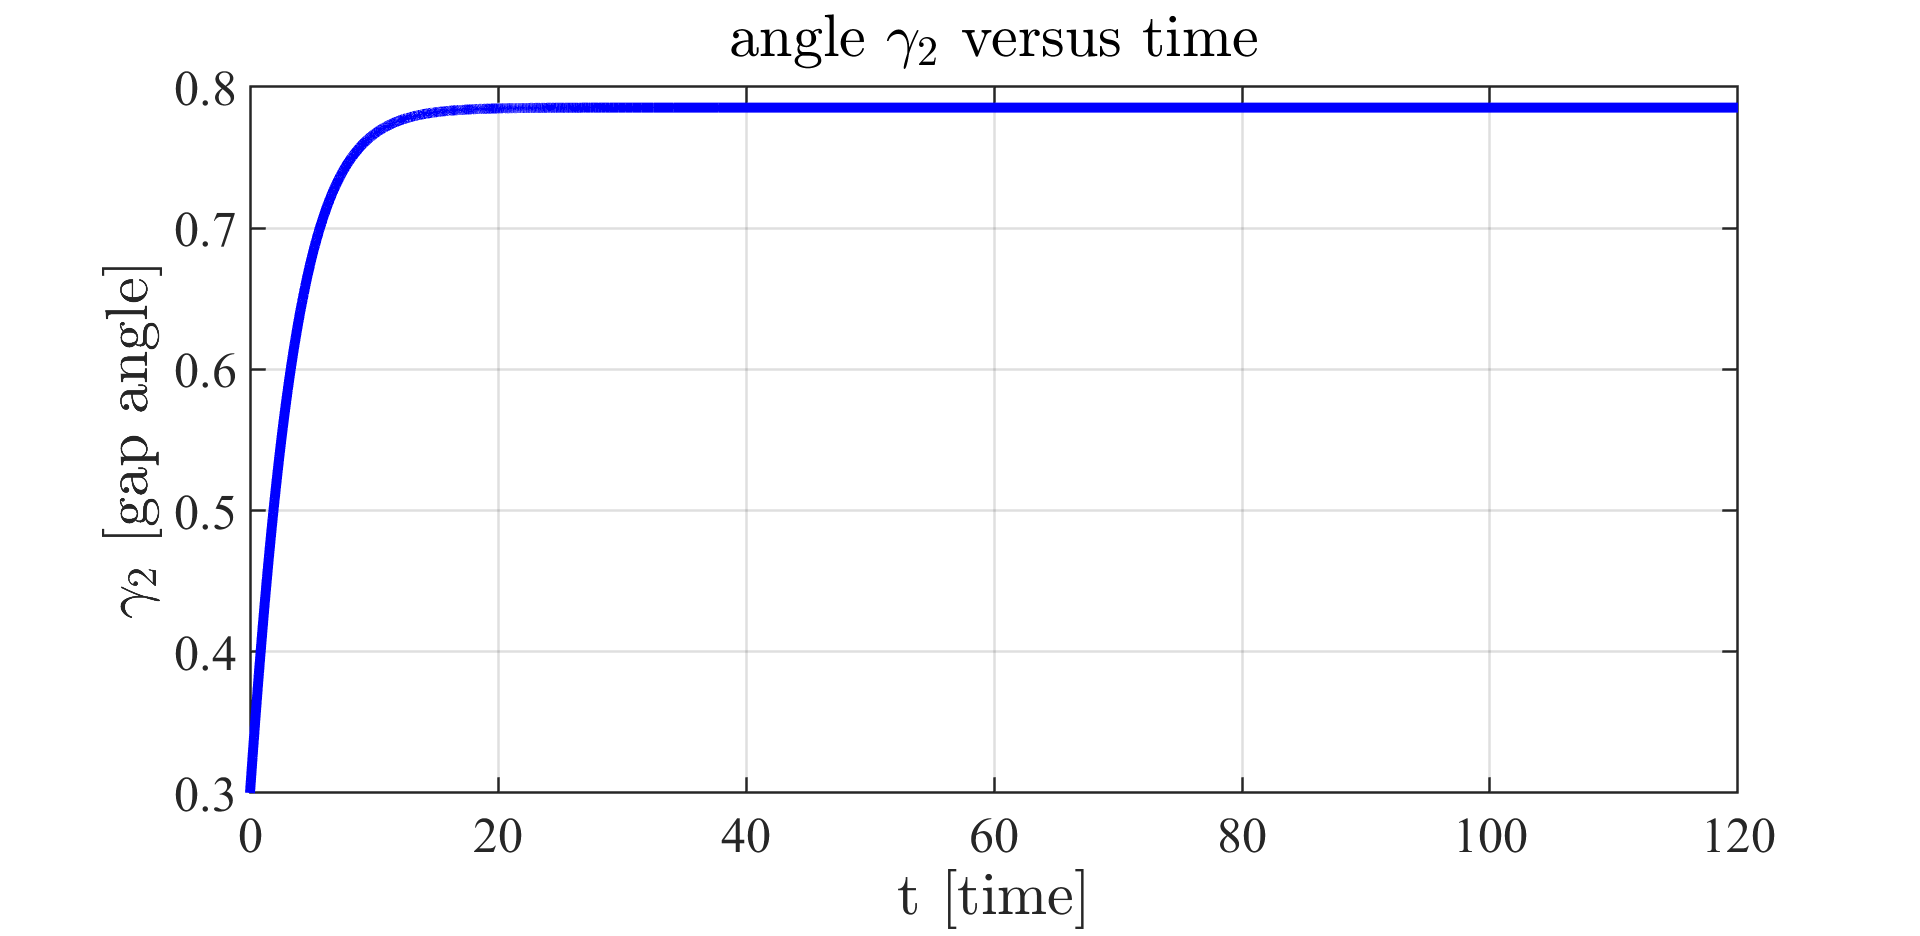
\includegraphics[width=11cm]{optstabilgamma2.png}\\
			\caption{Gap angle $\gamma_2$ versus time}
			\label{optcontrollab4}
		\end{center}
	\end{figure}
	
	\begin{figure}[htp]
		\begin{center}
			% Requires \usepackage{graphicx}
			% replace aims_logo.eps by your figure file name
			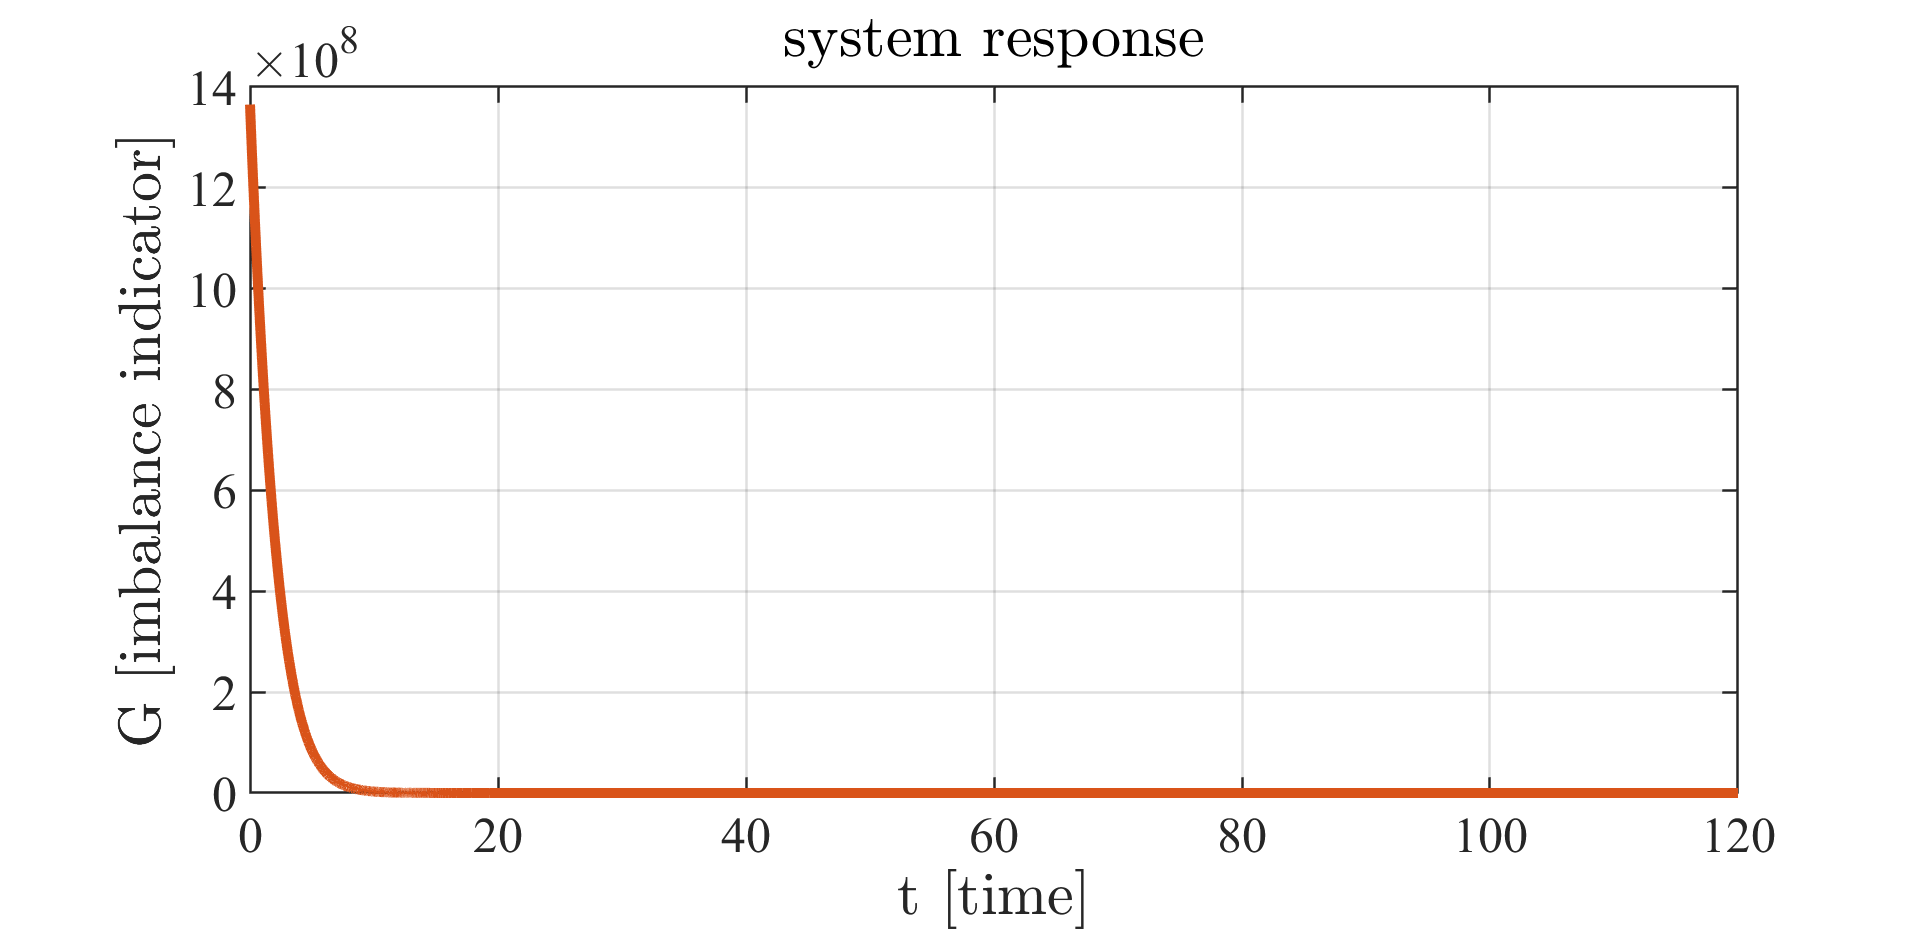
\includegraphics[width=11cm]{systemresponse.png}\\
			\caption{The imbalance indicator $G$ along the computed trajectory versus time.}
			\label{systemresponse}
		\end{center}
	\end{figure}

\newpage

\section*{Appendix}

\subsection{IPOpt-AMPL code}

As announced, we provide the \verb!IPOpt!-\verb!AMPL! code related to the minimization problem \eqref{functional}.

\begin{verbatim}
#parameters for the algorithm execution.
param pi = 4*atan(1);
param Nt = 10000;
param T = 120;
param dt = T/(Nt);

#physical parameters.
param m1 = 1;
param m2 = 1;
param a = 1;
param b = 1;
param r1 = 1;
param r2 = 1;
param omega = 2000*(2*pi)/60;
param Fx = -2*m1*r1*omega^2;
param Fy = -2*m2*r2*omega^2;
param Nx = 0;
param Ny = 0;
param F1x = (b*Fx-Ny)/(a+b);
param F1y = (b*Fy+Nx)/(a+b);
param F2x = (a*Fx+Ny)/(a+b);
param F2y = (a*Fy-Nx)/(a+b);
#param ss = [0;pi;0;pi];
#WARNING:
#The condition below must be fulfilled.
#m_1r_1 > \frac{\sqrt{F_{1,x}^2+F_{1,y}^2}}{2\omega^2}\hspace{0.3 cm}\mbox{and}\hspace{0.3 cm}m_2r_2> \frac{\sqrt{F_{2,x}^2+F_{2,y}^2}}{2\omega^2},

#weighting parameters.
param beta = 0.25*(2*omega^2)^(-2); #omega^4*(1000/120);

var Phi {i in 0..Nt, j in 1..4};  # Phi(t), state
var psi {i in 0..Nt-1, j in 1..4}; # psi(t), control, default 0;

minimize cost: sum {i in 0..Nt-1} (0.5*dt*(psi[i,1]^2+psi[i,2]^2+psi[i,3]^2+psi[i,4]^2)+(beta/(2))*dt*((2*m1*r1*omega^2*cos(Phi[i,2])*cos(Phi[i,1])+F1x)^2+(2*m1*r1*omega^2*cos(Phi[i,2])*sin(Phi[i,1])+F1y)^2)+(beta/(2))*dt*((2*m2*r2*omega^2*cos(Phi[i,4])*cos(Phi[i,3])+F2x)^2+(2*m2*r2*omega^2*cos(Phi[i,4])*sin(Phi[i,3])+F2y)^2));

subject to Phi_dyn_one {i in 1..Nt}:
((Phi[i,1]-Phi[i-1,1])/(dt)) = psi[i-1,1];
subject to Phi_dyn_two {i in 1..Nt}:
((Phi[i,2]-Phi[i-1,2])/(dt)) = psi[i-1,2];
subject to Phi_dyn_three {i in 1..Nt}:
((Phi[i,3]-Phi[i-1,3])/(dt)) = psi[i-1,3];
subject to Phi_dyn_four {i in 1..Nt}:
((Phi[i,4]-Phi[i-1,4])/(dt)) = psi[i-1,4];

subject to initial_condition_one: Phi[0,1] = 1;
subject to initial_condition_two: Phi[0,2] = 0.3;
subject to initial_condition_three: Phi[0,3] = 0.6;
subject to initial_condition_four: Phi[0,4] = 0.3;

option solver ipopt;
option ipopt_options "max_iter=2000 linear_solver=mumps halt_on_ampl_error yes";
solve;


printf: " # cost = %24.16e\n", cost; # > out_MMarposs1.txt;
printf: " # T = %24.16e\n", T; # > out_MMarposs1.txt;
printf: " # Nt = %d\n", Nt; # >> out_MMarposs1.txt;
printf: " # Data\n"; # >> out_MMarposs1.txt;
printf {i in 0..Nt}: " %24.16e\n", Phi[i,1]; # >> out_MMarposs1.txt;
printf {i in 0..Nt}: " %24.16e\n", Phi[i,2]; # >> out_MMarposs1.txt;
printf {i in 0..Nt}: " %24.16e\n", Phi[i,3]; # >> out_MMarposs1.txt;
printf {i in 0..Nt}: " %24.16e\n", Phi[i,4]; # >> out_MMarposs1.txt;
printf: " # Imbalance indicator evaluated at (Phi[Nt,1],Phi[Nt,2],Phi[Nt,3],Phi[Nt,4])\n"; # > out_MMarposs1.txt;
printf: " %24.16e\n", ((2*m1*r1*omega^2*cos(Phi[Nt,2])*cos(Phi[Nt,1])+F1x)^2+(2*m1*r1*omega^2*cos(Phi[Nt,2])*sin(Phi[Nt,1])+F1y)^2)+((2*m2*r2*omega^2*cos(Phi[Nt,4])*cos(Phi[Nt,3])+F2x)^2+(2*m2*r2*omega^2*cos(Phi[Nt,4])*sin(Phi[Nt,3])+F2y)^2); # >> out_MMarposs1.txt;



end;
\end{verbatim}

\verb!IpOpt!-\verb!AMPL! codes can be run for free in NEOS solvers\\
\url{https://neos-server.org/neos/solvers/nco:Ipopt/AMPL.html}
	
	
	
	
	%%The title of your section 3
	%\section{How to align the math formulas}
	%
	%\begin{theorem} \label{result2}
	%        Content of your theorem.
	%\end{theorem}
	%
	%In the proof below, we would like to show you how to align the math
	%formulas:
	%\begin{proof}[Proof of Theorem \ref{result2}]
	%    Please refer to the following example and align your math formulas:
	%\begin{equation}\label{Multi}
	% \begin{split}
	%    \eps{\theta} \wedge d\eps{\theta}^{n-1} =& (\theta_0 + \ep \alpha)
	%    \wedge (d(\theta_0 + \ep \alpha))^{n-1} \quad \text{since } d\alpha = 0\\
	%    =& (\theta_0 + \ep \alpha) \wedge
	%    (d\theta_0)^{n-1} + \theta_0 \wedge d\theta_0^{n-1} - \ep d(\alpha \wedge
	%    \theta_0 \wedge d\theta_0^{n-2})\\
	%    &  + \theta_0 \wedge d\theta_0^{n-1} + \ep \alpha \wedge
	%    d\theta_0^{n-1}  \\
	%    =& \theta_0 \wedge d\theta_0^{n-1} - \ep d(\alpha \wedge
	%    \theta_0 \wedge d\theta_0^{n-2}),
	% \end{split}
	%\end{equation}
	%
	%It also can be aligned in the following way:
	%
	%\begin{equation}\label{Multi}
	% \begin{split}
	%    &\eps{\theta} \wedge d\eps{\theta}^{n-1} \\
	%    =& (\theta_0 + \ep \alpha)
	%    \wedge (d(\theta_0 + \ep \alpha))^{n-1} \quad \text{since } d\alpha = 0\\
	%    =& (\theta_0 + \ep \alpha) \wedge
	%    (d\theta_0)^{n-1} + \theta_0 \wedge d\theta_0^{n-1} - \ep d(\alpha \wedge
	%    \theta_0 \wedge d\theta_0^{n-2})\\
	%    &  + \theta_0 \wedge d\theta_0^{n-1} + \ep \alpha \wedge
	%    d\theta_0^{n-1}  \\
	%    =& \theta_0 \wedge d\theta_0^{n-1} - \ep d(\alpha \wedge
	%    \theta_0 \wedge d\theta_0^{n-2}),
	% \end{split}
	%\end{equation}
	%
	%\newpage
	%
	%Here is another example if the math expression in [ ] exceeds one
	%line:
	%
	%\begin{equation}\label{Equ3}
	% \begin{split}
	%\int_0^T |u_0(t)|^2dt  \leq& \delta^{-1} [\int_0^T
	%(\beta(t)+\gamma(t)) dt\\
	%&  \quad\quad+T^{\frac{2(p-1)}{p}}(\int_0^T
	%|\cdot{u}_0(t)|^pdt)^{\frac{2}{p}}
	% +T^{\frac{2(p-1)}{p}}(\int_0^T |\cdot{u}_0(t)|^pdt)^{\frac{2}{p}}].
	% \end{split}
	%\end{equation}
	%
	% Please use the displaystyle if your formulas fully
	%occupy a paragraph, while use textstyle among the text.
	%
	%For two equations:
	%\begin{align*}
	%A &= \theta_0 \wedge d\theta_0^{n-1} - \ep d(\alpha \wedge \theta_0 \wedge d\theta_0^{n-2})\\
	%B&=\theta_1 \wedge d\theta_1^{n-1} - \ep d(\alpha \wedge \theta_1
	%\wedge d\theta_1^{n-2})
	%\end{align*}
	%Please align your formulas nicely according above examples. Thanks.
	%\end{proof}
	
	%For acknowledgements section, please don't number the section, please begin it with \section*{Acknowledgements}
	%\section*{Acknowledgments} We would like to thank you for \textbf{following [ADD]
	%the instructions above} very closely in advance. It will definitely
	%save us lot of time and expedite the process of your paper's
	%publication.
	
	% You may incorporate your references as follows in your main tex file.
	% Using BibTex is not recommended but can be handled.
	
	\bibliography{my_references}
	\bibliographystyle{siam}
	
	\medskip
	% The data information below will be filled by AIMS editorial staff
	Received xxxx 20xx; revised xxxx 20xx.
	\medskip
	
\end{document}
